
\begin{frame}{Equações Diferenciais Ordinárias (EDOs)}
    \begin{itemize}
        \item Usadas para estudar o comportamento populacional ao longo do tempo;
        \item Diversas aplicações em várias áreas do conhecimento; 
        \item Cada equação descreve a concentração de uma população diferente;
    \end{itemize}

    \begin{columns}
        \begin{column}{.4\textwidth}
            \begin{equation}
                \begin{array}{lr}
                    \frac{dN_1}{dt} = r_1.N_1(1 - W_{11}.N_1 - W_{21}.N_2)
                    \\
                    \\
                    \frac{dN_2}{dt} = r_2.N_2(1 - W_{22}.N_2 - W_{12}.N_1)
                \end{array}
            \end{equation}
        \end{column}

        \begin{column}{.6\textwidth}
            \begin{figure}
                \centering
                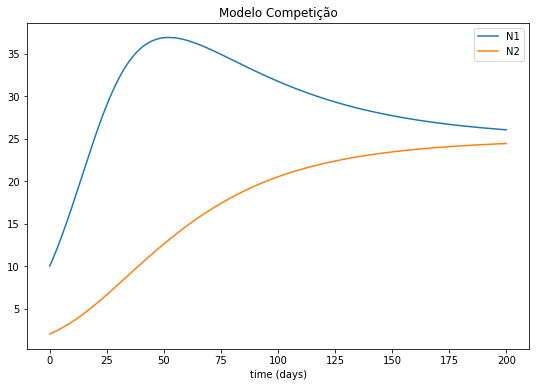
\includegraphics[height=.7\textheight]{beamerthemesrc/images/ode}
            \end{figure}
        \end{column}
    \end{columns}
\end{frame}

\begin{frame}{EDO — Modelo Predador-Presa}
    Um modelo clássico da literatura é o modelo Predador-Presa. Este modelo descreve o comportamento de duas populações, $H$ e $P$, que possuem uma uma relação de predação entre si. 

    \begin{columns}
        \begin{column}{.3\textwidth}
            \begin{equation}\label{eq:predadorpresa}
                \begin{array}{lr}
                    \frac{dH}{dt} = r.H - a.H.P
                    \\
                    \\
                    \frac{dP}{dt} = b.H.P - m.P
                \end{array}
            \end{equation}
        \end{column}
        \begin{column}{.6\textwidth}
            Na equação, temos que
            \[
            \begin{array}{lr}
                H & \text{Presa}\\
                P & \text{Predador}\\
                r & \text{Taxa de reprodução da presa}\\
                m & \text{Taxa de mortalidade dos predadores}\\
                a & \text{Taxa de predação}\\
                b & \text{Taxa de reprodução dos predadores}\\
                \end{array}.
            \]
        \end{column}
    \end{columns}

\end{frame}
    
\begin{frame}{Programação visual}
    \begin{itemize}
        \item É uma maneira do usuário programar a máquina por meio de elementos gráficos que abstraem instruções do computador. \item Os elementos podem representar múltiplas operações por vez, com o objetivo de facilitar a programação.
        \item Exemplos: GRAIL, Scratch, Logisim, Blender. 
        \item Editores baseados em nós são muitos usados porque possuem uma representação natural para operações complexas que combinam um conjunto de entradas para gerar uma ou mais saídas. 
    \end{itemize}    
\end{frame}

\begin{frame}{Programação visual}
    \item GRaIL — 1968:
    \href{https://www.youtube.com/watch?v=QQhVQ1UG6aM}{
        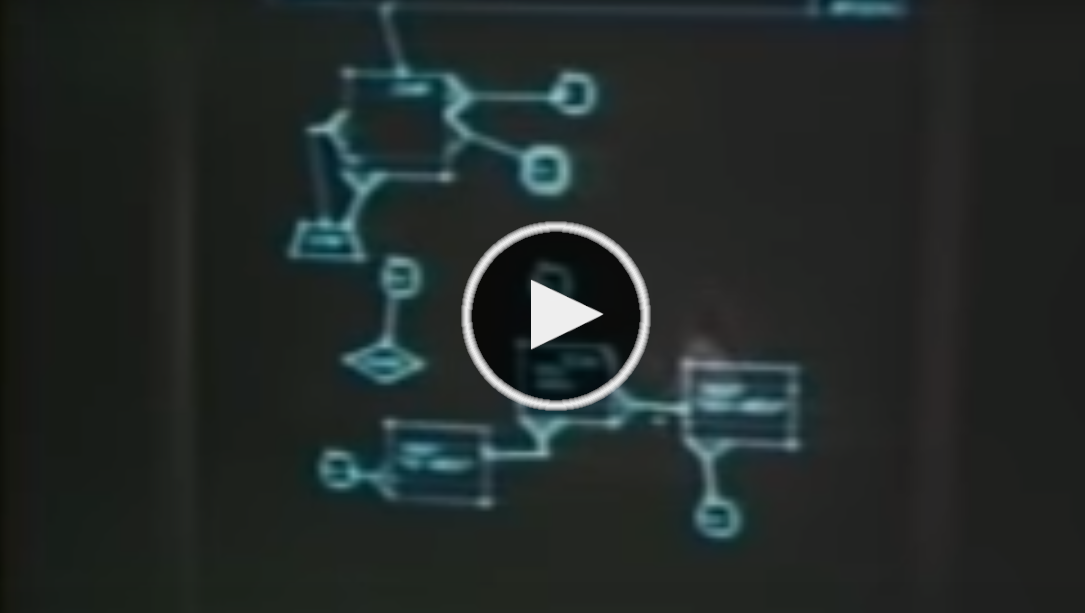
\includegraphics[width=\textwidth, height=\textheight, keepaspectratio=true]{beamerthemesrc/images/video-thumb.png}
    }
\end{frame}

\begin{frame}{Geração de código}
    \begin{itemize}
        \item Recebe como entrada uma Representação Intermediária (RI) e gera como saída um código na linguagem alvo (por exemplo, Python).
    \end{itemize}    
\end{frame}

\begin{frame}{Geração de código baseada em \textit{templates}}
    \begin{itemize}
        \item 
    \end{itemize}    
\end{frame}